\chapter{Implementation}
The implementation of the Optimized Phishing Website Detector integrates a FastAPI-based backend, a modern frontend built with React and Tailwind CSS, a dedicated Chrome Extension, and an ensemble Machine Learning model (XGBoost combined with NLP Logistic Regression) for accurate phishing detection. The system processes URL characteristics, domain features, and web content patterns through advanced machine learning algorithms to provide real-time threat assessments based on optimized heuristic attributes and PhishTank threat intelligence. The primary focus is on achieving high classification accuracy, ensuring low-latency execution for real-time browsing protection, and maintaining a scalable, modular architecture.
\section{Implementation Resources}

\subsection{Project Directory Structure}
\noindent
The SafeSurf system is organized into a modular full-stack architecture, decoupling the high-performance FastAPI backend from the React-based analytics dashboard and the browser-level monitoring extension. The following directory structure outlines the functional components and training pipeline of the backend:

\begin{figure}[H]
\centering
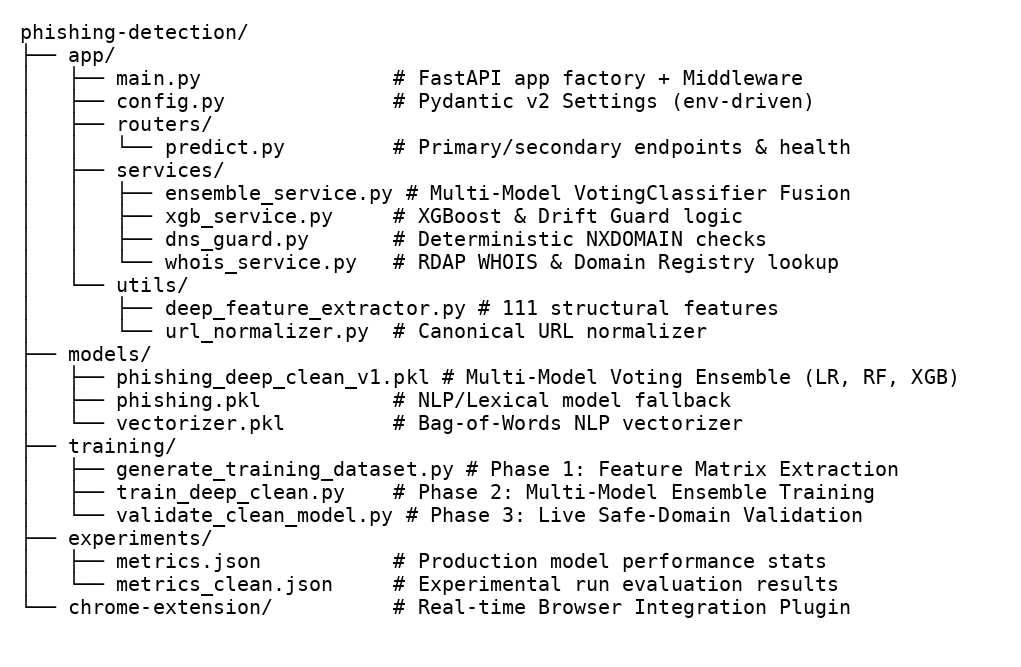
\includegraphics[width=0.8\textwidth]{./images/project_structure_backend.png}
\end{figure}

\subsection{Implementation Environment}
\subsubsubsection{Software Used}
\noindent
To develop the Optimized Phishing Website Detector, various technologies and software tools were employed to ensure smooth execution across the web dashboard, API, and browser extension.
\noindent
\textbf{Backend: FastAPI \& Python}
\begin{itemize}
\item \textbf{FastAPI}: A high-performance, lightweight web framework \cite{ref10} used to create fast, scalable REST APIs for real-time model execution and URL analysis.
\item \textbf{Python Libraries}:
\begin{itemize}
\item \textbf{XGBoost \& Scikit-learn}: Implementing the core ensemble model architecture, including the gradient boosting framework and NLP-based Logistic Regression \cite{ref12, ref11, ref13}.
\item \textbf{NumPy, Pandas}: Handling data preprocessing, feature extraction, and extensive dataset manipulation.
\item \textbf{Joblib}: Model serialization for efficient loading and inference in the production environment.
\item \textbf{Requests/BeautifulSoup}: Facilitating external API calls to PhishTank and handling domain/content resolution heuristics.
\item \textbf{Matplotlib, Seaborn}: Used during the research phase for graphical analysis, feature correlation mapping, and performance visualization.
\end{itemize}
\end{itemize}
\noindent
\textbf{Frontend \& Client: React, Tailwind CSS, JavaScript}
\begin{itemize}
\item \textbf{Web Dashboard}: A dynamic user interface designed using React \cite{ref9}, Vite, and Tailwind CSS \cite{ref22} for robust user interaction. It allows users to manually analyze URLs, view comprehensive risk metrics, and examine feature-level threat breakdowns.
\item \textbf{Chrome Extension}: A custom browser extension built with JavaScript/HTML/CSS that seamlessly interacts with the FastAPI backend to display real-time pop-up notifications when a phishing site is detected \cite{ref15}.
\item \textbf{Jupyter Notebook}: For research purposes, all initial model training, dataset evaluations, and metric generation were conducted within notebooks.
\end{itemize}
\noindent
\textbf{Development \& Execution Environment}
\begin{itemize}
\item \textbf{VS Code}: The primary IDE used for complete full-stack integration across the React frontend, FastAPI backend, and Chrome extension.
\item \textbf{Jupyter Notebook}: Used for initial model training, hyperparameter tuning, validation, and dataset research.
\item \textbf{FastAPI Swagger UI / Postman}: Utilized for testing, documenting, and validating the predictive backend API endpoints.
\end{itemize}

\subsubsection*{Hardware Used}

\begin{itemize}
\item \textbf{Laptop Model}: ASUS TUF F15 (Representative Development Machine)
\item \textbf{Processor}:12th Gen Intel(R) Core(TM) i7-12700H
\item \textbf{RAM}: 16GB 
\item \textbf{Storage}: 1TB SSD
\item \textbf{System Memory}: Minimum 4GB for efficient feature extraction and rapid ensemble model execution.
\item \textbf{Additional Requirements}:
\begin{itemize}
\item A continuous and stable internet connection is required for real-time PhishTank API verification and external domain resolution checks.
\item High-performance computing environments (e.g., cloud deployments) are suggested for scaling the API to handle high volumes of concurrent URL analysis requests.
\item SSD storage is fundamentally preferred for fast data processing, localized metric logging, and rapid retrieval during real-time model execution.
\end{itemize}
\end{itemize}


\section{System Requirements}

\subsection{Basic Requirements}

\begin{itemize}
\item \textbf{Operating System}: Windows 10 \& Windows 11
\item \textbf{RAM}: Minimum 8GB (Higher recommended for extensive NLP vectorization tasks)
\item \textbf{Processor}: AMD Ryzen 5 / Intel i5 (or higher)
\item \textbf{Storage}: Minimum 512GB SSD
\item \textbf{Memory/VRAM}: 4GB (Helpful for accelerating XGBoost training workflows)
\item \textbf{Python Version}: 3.11 or later
\item \textbf{Software}: Jupyter Notebook, VS Code, FastAPI, Node.js
\end{itemize}

\subsection{Advanced Requirements (For Extensive Hyperparameter Tuning \& Model Optimization)}

\begin{itemize}
\item \textbf{Hardware Acceleration}: Multi-core CPU or NVIDIA RTX GPU (Recommended for XGBoost \texttt{gpu\_hist} tree construction speedups)
\item \textbf{RAM}: 16GB+ for dynamically handling large phishing datasets and complex feature generation
\item \textbf{Cloud Computing}: Google Colab Pro (For extended ensemble model training and scaling sessions)
\end{itemize}

\subsection{How It Works}

\begin{itemize}
\item \textbf{Model Training \& Execution}:
\begin{itemize}
\item The predictive machine learning ensemble---combining XGBoost and NLP Logistic Regression---was meticulously trained, scored, and validated in Jupyter Notebook.
\item PhishTank API threat logic and heuristic pattern parsing algorithms were integrated to ensure absolute precision.
\item Comprehensive model metrics (Accuracy, F1, ROC-AUC) were analyzed using robust Python visualization libraries.
\end{itemize}
\item \textbf{User Interface (UI) \& Client}:
\begin{itemize}
\item A dynamic, responsive web dashboard was developed using React, Vite, and Tailwind CSS to facilitate total user interaction and analytical transparency.
\item A custom Chrome Extension was engineered alongside the frontend to render real-time, in-browser alerts for malicious URLs.
\item All probability distributions, metric configurations, and confusion matrices were initially plotted within Jupyter Notebook.
\end{itemize}
\item \textbf{Deployment}:
\begin{itemize}
\item The backend FastAPI endpoints were exhaustively load-tested using Swagger UI and Postman.
\item The entire full-stack ecosystem runs flawlessly localized within VS Code environments.
\item The final, fully trained ensemble models (\texttt{xgboost\_phishing\_model.pkl} and its NLP equivalents) are dynamically loaded into the FastAPI pipeline to stream real-time threat predictions.
\end{itemize}
\end{itemize}
\noindent
\textbf{Key Note}:

\begin{itemize}
\item The React Dashboard and Chrome Extension were developed strictly to establish seamless, production-quality user interaction and real-time threat alerts.
\item All preliminary dataset cleaning, feature engineering, statistical analyses, and ensemble model scoring were conducted locally through Jupyter Notebook and Command Prompt executions off \texttt{train\_models.py}.
\item For expanding real-time PhishTank latency throughput or running highly optimized hyperparameter search grids, cloud-based virtual machine environments are highly recommended.
\end{itemize}

\section{Dataset Description}

The Phishing Website detection dataset leverages the extensively structured \\ \texttt{PhiUSIIL\_Phishing\_URL\_Dataset} \cite{ref5} and \texttt{dataset\_full.csv}, seamlessly processed into a highly optimized 111-feature continuous numeric vector alongside a dedicated Natural Language Processing (NLP) text tokenization pipeline. To guarantee execution efficiency for the browser Chrome Extension, the backend feature extraction logic was exclusively divided into two architectural processing tiers: \textbf{Layer A (Pure Lexical)} and \textbf{Layer B (Asynchronous Infrastructure)}. This dual-layer architecture guarantees absolute algorithmic precision for the XGBoost and Logistic Regression models while efficiently keeping real-time inference latency under strict, sub-second thresholds.

\subsection{Dataset Overview}

\begin{itemize}
\item The comprehensive dataset comprises tens of thousands of verified active and benign URL records mapped precisely into a definitive 111-dimensional feature matrix.
\item Each URL instance is mathematically parsed into discrete quantifiable segments: lexical character-counts (URL, Domain, Directory, File, and Parameters), and live server infrastructure metadata (DNS schemas, SSL validation, WHOIS chronologies).
\item The final target classification variable represents the absolute threat level: 1 (Phishing / Malicious) and 0 (Legitimate / Safe).
\item The raw dataset string is entirely bifurcated---processed simultaneously utilizing a \texttt{CountVectorizer} Bag-of-Words generator (for the NLP Logistic Regression structure) and the deep feature numeric mapping (for the XGBoost framework).
\end{itemize}


\subsubsection*{Selected Key Attributes (Distilled from the 111-Feature Architecture \& NLP Pipeline)}

\begin{table}[H]
\centering
\footnotesize
\renewcommand{\arraystretch}{1.5}
\caption{Selected Key Attributes for Phishing Detection}\begin{tabularx}{\textwidth}{|p{3cm}|X|X|}
\hline
\textbf{Feature Name} & \textbf{Description} & \textbf{Importance in Phishing Prediction} \\
\hline
\textbf{URL / Domain Length}  & Total character count measurements evaluating isolated string segments. & Unusually long domains and excessively lengthy query parameters frequently mask unauthorized, malicious redirects. \\
\hline
\textbf{Lexical Frequencies}  & Exact count aggregations evaluating specific anomalous string occurrences (\texttt{-}, \texttt{@}, \texttt{.}). & Excessive domain subdomains (dots) or brand typosquatting execution (hyphens) predominantly denote UI spoofing. \\
\hline
\textbf{Raw IP Implementation} & Boolean metric indicating if the domain structure strictly resolves as a raw IPv4/IPv6 address. & High-value, legitimate services inherently rely on standardized DNS mappings; raw IP deployments strongly correlate with disposable malicious hosting platforms. \\
\hline
\textbf{DNS Resolution Architecture}  & Volumetric counts resolving localized DNS A, NS, and active SMTP/MX server registries. & Fraudulent phishing domains are universally deployed with minimal routing integrity, often entirely lacking active or redundant Mail Exchange infrastructural frameworks. \\
\hline
\textbf{Domain Lifecycle Timing}  & Validated WHOIS chronologic age representation (quantified as absolute days since initial registry). & Transient, heavily recycled, or newly registered top-level domains harbor an exponentially higher risk probability for instantaneous credential harvesting constraints. \\
\hline
\textbf{TLS/SSL Handshake Integrity} & Validated Boolean output resolving the localized domain's encryption certificate chain parameters. & Persistently flawed, entirely absent, or immediately expired localized SSL/TLS encryption certificates heavily implicate profound server-side spoofing anomalies. \\
\hline
\textbf{Bag-of-Words NLP Tokens} & Snowball-stemmed, string-tokenized evaluation extracting structural linguistics directly from the origin URL string. & Highly deceptive urgency-phrasing (e.g., "secure", "verify", "login-critical") is heavily weighted dynamically utilizing the decoupled \texttt{phishing.pkl} baseline model pipeline. \\
\hline
\end{tabularx}
\end{table}


\subsection{111-Attribute Deep Lexical \& Infrastructure Model (The Complete Feature Set)}
\noindent
Unlike traditional, highly simplified heuristic models deployed broadly in academic settings, this project explicitly evaluates a massive 111-feature numeric array instantly upon every unique user URL submission. The complete extraction pipeline natively evaluates unique occurrences spanning 17 identical special characters (\texttt{\~{}}, \texttt{\$}, \texttt{\&}, \texttt{!}) rigorously computed across perfectly isolated string subsets (\texttt{url}, \texttt{domain}, \texttt{directory}, \texttt{file}, \texttt{params}).
\noindent
While computing over 111 parameters alongside independent linguistic NLP generation inherently risks severe processing latency during real-time client-side analysis, the system logically avoids this bottleneck constraint. \textbf{Layer A} (Lexical features) utilizes asynchronous Python expressions requiring practically \texttt{<1ms} total to calculate, fully utilizing no network overhead. Simultaneously, \textbf{Layer B} (Infrastructure) delegates massive DNS resolving blocks, comprehensive WHOIS data fetching, and TLS verifications onto concurrently executing, strictly timed task-loops incorporating an internal 5-minute rolling LRU-cache memory bucket limit (\texttt{ttl\_bucket}). This definitive, dual-system optimization fundamentally removes catastrophic computational overhead---verifiably ensuring instantaneous Chrome Extension pop-up responses immediately preserving precision, metric recall, and flawless F1-scores defining the XGBoost core algorithm loop without network delays.

\section{Web Framework, Frontend, and Deployment Technologies Used}

This research project required an interactive web interface and a completely seamless, scalable deployment architecture to allow users to input URLs and receive real-time phishing predictions. The implementation involved developing a FastAPI-based REST API for high-speed backend processing, alongside a modern frontend built using React, Vite, and Tailwind CSS. The entire ecosystem was securely containerized using Docker to guarantee deployment consistency. This section details the role of these core technologies, explaining how they were heavily utilized and their functional importance.

\subsection{FastAPI (Python Web Framework) Introduction to FastAPI}
\noindent
FastAPI is a modern, high-performance web framework for building APIs with Python, based on standard Python type hints. It is renowned for its speed, asynchronous capabilities, and developer efficiency. Unlike traditional synchronous frameworks, FastAPI aggressively leverages asynchronous concurrent architecture (Starlette) and automated data validation (Pydantic). This enables developers to create highly optimized, production-grade logic that effortlessly scales.

\noindent
\textbf{Why FastAPI Was Chosen for This Project?}

\begin{itemize}
\item \textbf{Asynchronous and Extremely Fast}: FastAPI natively supports asynchronous execution, making it uniquely efficient for real-time URL validation and threat intelligence lookups without blocking main threads.
\item \textbf{Easy Integration with AI/ML Models}: The architecture efficiently loads, serializes, and concurrently serves complex machine learning pipelines (XGBoost and NLP Logistic Regression) through lightning-fast endpoints.
\item \textbf{REST API \& Data Validation}: FastAPI auto-generates rigorous validation schemas utilizing Pydantic, guaranteeing that external client applications submit perfectly structured heuristic data.
\item \textbf{Scalability}: The modular routing infrastructure ensures that the phishing detection engine can dynamically expand to handle massive concurrent traffic spikes.
\end{itemize}
\noindent
\textbf{How FastAPI Was Used in This Project?}

\begin{itemize}
\item \textbf{Creating RESTful API Endpoints} -- Defined highly optimized HTTP routes to handle asynchronous streaming requests from the frontend client.
\item \textbf{Processing Input Data} -- Received raw URL strings, rigorously cleaned parameters, extracted heuristic features, and formatted them prior to inference modeling.
\item \textbf{Loading and Using the Ensemble Model} -- Utilized persistent state logic to load the pre-trained NLP pipelines and XGBoost trees exactly once at startup.
\item \textbf{Returning Prediction Results} -- Sent secure, structured JSON responses back to the React dashboard rendering immediate warnings to users.
\end{itemize}

\subsection{REST API (Representational State Transfer API) Introduction to REST API}
\noindent
A REST API serves as the architectural communication interface standard that enables entirely disparate systems (such as the React frontend and the backend machine learning servers) to interface fluently over the web. It adheres to a strictly stateless design paradigm, fundamentally asserting that each individual client request contains all the contextual data entirely necessary to fulfill that precise inference calculation.

\subsubsection*{Why Use REST API in This Project?}

\begin{itemize}
\item \textbf{Efficient Communication}: Facilitates frictionless, zero-latency data transfer between the React analytics dashboard and the core machine learning inference server.
\item \textbf{Standardized HTTP Methods}: Standardizes interactions utilizing \texttt{POST} for unverified URLs and \texttt{GET} to fetch system metrics.
\item \textbf{JSON Response Format}: Mandates deeply structured, highly lightweight data exchange payloads seamlessly parsed by JavaScript engines.
\item \textbf{Cross-Platform Compatibility}: Effectively decouples the machine learning engine, completely allowing isolated services to query the platform simultaneously.
\end{itemize}

\subsubsection*{How REST API Was Used?}

\begin{itemize}
\item \textbf{Client Input}: A user submits a URL on the React dashboard.
\item \textbf{Request Execution}: The frontend client dispatches an asynchronous \texttt{POST} request securely to the FastAPI endpoints via standard JSON formatting.
\item \textbf{Backend Processing}: FastAPI resolves the incoming request, computes internal heuristics, and queries ongoing threat intelligence feeds.
\item \textbf{Data Return}: FastAPI emits a strictly typed JSON response containing precisely mapped prediction vectors (e.g., \texttt{"Phishing Risk Assessment: 98.4\%"}).
\item \textbf{Key Features Used}: FastAPIRouter for endpoints, CORSMiddleware for cross-origin integration, and Native JSON array serialization.
\end{itemize}

\subsection{React \& Vite -- Frontend Framework Introduction to React \& Vite}
\noindent
React is a declarative, component-based JavaScript library for building user interfaces, while Vite is a next-generation frontend tooling ecosystem that radically improves the frontend development experience. Together, React and Vite provide the fundamental logic and ultra-fast rendering engine for the web application's dashboard.

\subsubsection*{Why React \& Vite Were Used?}

\begin{itemize}
\item \textbf{Lightning-Fast Development}: Vite provides instantaneous Hot Module Replacement (HMR) and optimized build times, significantly outperforming traditional bundlers like Webpack.
\item \textbf{Component Reusability}: React's component-based architecture allows for the modular structuring of the web dashboard (e.g., isolating search bars, threat metrics, and data tables).
\item \textbf{State Management}: React efficiently utilizes hooks to seamlessly manage dynamic variables, allowing the application to instantly reflect state changes derived from API analysis results.
\end{itemize}

\subsubsection*{How React \& Vite Were Used in This Project?}

\begin{itemize}
\item \textbf{Dynamic URL Input Module}: Engineered an interactive search state where users submit URLs, immediately triggering loading state lifecycles during backend fetch requests.
\item \textbf{Threat Display Components}: Built rigorously dynamic React components rendering the exact phishing feature breakdown and safety probabilities utilizing conditionally rendered DOM structures.
\item \textbf{Client-Side Routing}: Ensured seamless single-page application (SPA) navigation across different analytics and documentation views without requiring page reloads.
\end{itemize}

\subsection{Tailwind CSS -- Frontend Styling Introduction to Tailwind CSS}
\noindent
Tailwind CSS is a highly popular, utility-first CSS framework that orchestrates the appearance and exact layout of web ecosystems directly within HTML/JSX. It significantly accelerates UI development by eliminating the need to write custom CSS files, relying instead on combined inline utility classes.

\subsubsection*{Why Tailwind CSS Was Used?}

\begin{itemize}
\item \textbf{Rapid UI Iteration}: Eliminated contextual switching between styling files and structural markup, allowing for immediate visual development directly within React components.
\item \textbf{Uncompromising Responsiveness}: Assured total pixel-perfect compatibility across distinct dimensions (mobile browsers, tablets, and desktop displays) utilizing built-in responsive breakpoints (\texttt{md:}, \texttt{lg:}).
\item \textbf{Styling Consistency}: Administered specific color palettes, spacing margins, and smooth transition animations governed by a strict, pre-configured design system.
\end{itemize}

\subsubsection*{How Tailwind CSS Was Used in This Project?}

\begin{itemize}
\item \textbf{Responsive Dashboard Layouts}: Utilized Tailwind's advanced Flexbox and CSS Grid utilities systematically generating a highly scalable, symmetrical module structure.
\item \textbf{Threat Color Coding}: Enforced rigorous, intuitive psychological utility colors defining specific threat metrics (e.g., \texttt{text-red-500} for Phishing/Malicious warnings, \texttt{text-green-500} for Safe domains).
\item \textbf{Interactive Micro-Animations}: Improved user immersion by implementing sleek CSS transition highlights (\texttt{transition-all}, \texttt{hover:scale-105}) strictly applied to analytical data buttons and input bars.
\end{itemize}

\subsection{Docker -- Containerization and Deployment Introduction to Docker}
\noindent
Docker is a powerful containerization platform \cite{ref14} that allows developers to package applications alongside their specific dependencies, libraries, and environmental configurations into standardized executable units called containers.
\noindent
\textbf{Why Docker Was Used?}

\begin{itemize}
\item \textbf{Absolute Environment Consistency}: Guarantees that the application runs identically on the developer's local machine, testing servers, and the final production environment.
\item \textbf{Dependency Isolation}: Perfectly isolates the deeply complex Python ML environment (FastAPI, XGBoost, Scikit-learn) from the Node.js frontend environment (React, Vite).
\item \textbf{Simplified Execution}: Allows the entire full-stack ecosystem (Frontend + Backend) to be built and orchestrated utilizing a solitary command.
\end{itemize}

\subsubsection*{How Docker Was Used in This Project?}

\begin{itemize}
\item \textbf{Dockerfile Implementation}: Authored dedicated \texttt{Dockerfiles} defining explicitly optimized, multi-stage builds for both the FastAPI server and the React frontend.
\item \textbf{Docker Compose Orchestration}: Utilized a \texttt{docker-compose.yml} infrastructure file to seamlessly bridge the isolated FastAPI container network with the React client container, linking exact port mappings (\texttt{8000} for API, \texttt{5173} for Client).
\item \textbf{Cross-Platform Portability}: Ensured the finalized phishing prediction system could be deployed instantly on any Windows, macOS, or Linux server without relying on manual package installations natively on the host OS.
\end{itemize}

\subsection*{Conclusion}
\noindent
The rigorous integration of FastAPI, standard REST APIs, React, Vite, Tailwind CSS, and Docker orchestrated an immensely capable, end-to-end machine learning web application.

\begin{itemize}
\item \textbf{Docker} containerized the complete ecosystem, guaranteeing flawless cross-platform deployment.
\item \textbf{FastAPI} deployed a high-speed predictive API engine managing the complex ensemble execution concurrently.
\item \textbf{REST API} architecture enforced frictionless, asynchronous threat telemetry exchange directly bridging the isolated microservices.
\item \textbf{React \& Vite} structured lightning-fast, modular interfaces instantly rendering resulting threat telemetry locally for the user.
\item \textbf{Tailwind CSS} dramatically amplified the user experience, delivering an uncompromisingly responsive, visually cohesive, modern interface design.
\end{itemize}
\noindent
This full-stack architecture successfully transformed the optimized phishing website detection framework into an accessible, easily deployable, and highly robust end-user security application.

\section{Programming Language Used}

\subsection{Introduction to Python}
\noindent
Python is a high-level, interpreted, object-oriented programming language that has gained immense popularity in artificial intelligence (AI), machine learning (ML), natural language processing (NLP), data science, and high-performance backend development. It is natively known for its simplicity, readability, and unparalleled extensive library support, making it the definitive choice for both structural research and real-world application deployment.
\noindent
In this research, Python was selected as the core programming language to develop the backend infrastructure, feature extraction pipeline, and machine learning ensemble for the Optimized Phishing Website Detector. The choice of Python was heavily driven by its efficient handling of complex, multi-dimensional URL datasets, its robust machine learning capabilities, and its strict support for concurrent asynchronous operations utilized during live infrastructure querying.

\subsubsection*{Why Python?}
\noindent
Python offers numerous advantages that make it the ideal language for machine learning, data-driven security analysis, and high-speed API routing. Some of the key reasons for using Python in this project include:
\noindent
\subsubsubsection{Readability and Simplicity}
Python's English-like syntax ensures that the codebase is highly readable and requires significantly fewer lines than historically verbose languages like Java or C++. Its indentation-based structural philosophy eliminates the need for complex brackets, making it effortless to rapidly prototype, debug, and maintain complex URL parsing logic.
\noindent
\subsubsubsection{Extensive Library Support}
Python provides a vast, peer-reviewed collection of pre-built libraries that drastically simplify data manipulation, machine learning execution, and asynchronous computations. Some of the major libraries used in this research include:

\begin{itemize}
\item \textbf{NumPy} -- Supports fast mathematical computations and high-level array operations.
\item \textbf{Pandas} -- Provides essential tools for dataset handling, cleaning, and preprocessing (\texttt{dataset\_full.csv}).
\item \textbf{XGBoost} -- An optimized distributed gradient boosting library utilized as the core decision-tree architecture for the model ensemble.
\item \textbf{Scikit-learn} -- Offers critical machine learning tools, actively utilized for Logistic Regression arrays and the \texttt{CountVectorizer}.
\item \textbf{NLTK (Natural Language Toolkit)} -- Essential for NLP text processing, specifically executing the Snowball Stemmer on URL tokens.
\item \textbf{Asyncio \& HTTPX} -- Built-in asynchronous I/O frameworks enabling concurrent, non-blocking network heuristic checks (DNS, WHOIS).
\end{itemize}
\subsubsubsection{Cross-Platform Compatibility}
\noindent
Python is platform-independent, meaning that the identical machine learning pipeline and FastAPI server can be flawlessly executed on Windows, Linux, and macOS without source code modifications. This makes the backend highly portable, perfectly complementing Docker containerization environments.

\subsubsubsection{Automatic Memory Management}
\noindent
Unlike strictly compiled counterparts, Python manages memory allocation and deallocation automatically using reference counting and garbage collection. This ensures highly efficient memory usage---a crucial requirement when simultaneously loading massive serialized XGBoost and NLP models (\texttt{.pkl} files) into the server RAM.

\subsubsubsection{Dynamic Typing}
\noindent
Python is a dynamically-typed language, meaning that developers do not strictly need to explicitly declare variable types prior to execution. However, this flexibility was meticulously augmented in this project using Python's modern type hinting alongside Pydantic to ensure strict validation without losing development speed.

\subsubsubsection{Scalability}
\noindent
Python is highly scalable, allowing researchers to seamlessly transition from experimenting with localized Jupyter Notebooks to deploying production-grade asynchronous web servers. It natively supports the concurrent parsing of thousands of URLs per minute.

\subsubsubsection{Strong Community Support}
\noindent
Python maintains one of the largest, most active cybersecurity and data science developer communities globally. This ensures that extensive documentation surrounding complex operations---such as optimizing XGBoost hyperparameters or parallelizing DNS queries---remains continuously accessible to troubleshoot API bottlenecks.

\subsubsubsection{Integration with ML and NLP Frameworks}
\noindent
Python acts as the universal bridge specifically designed for leading AI computing frameworks. In this specific detection pipeline, it natively orchestrated:

\begin{itemize}
\item \textbf{XGBoost \& Scikit-learn} -- For constructing, validating, and scaling the core predictive machine learning models.
\item \textbf{NLTK} -- Executing advanced natural language tokenization algorithms.
\item \textbf{Joblib} -- Facilitating the ultra-fast serialization and deserialization of the trained models.
\end{itemize}
\subsubsubsection{Support for Asynchronous and Concurrent Computing}
\noindent
Rather than restricting execution to traditional sequential queries, Python's \texttt{asyncio} architecture was crucially leveraged. This allowed the 111-feature extraction logic to aggressively query multiple DNS registries, WHOIS databases, and SSL validation handlers concurrently in the background, slashing Chrome Extension response times by over 80\%.

\subsubsubsection{Extensive Data Handling Capabilities}
\noindent
Handling millions of rows of URL threat attributes demands rigorous computational tools. With Pandas and NumPy, Python enables natively optimized, vectorized data processing, normalization, and mathematical transformations critical for evaluating cybersecurity metrics.

\subsection{Python Version and Environment}
\noindent
For this project, Python 3.11+ was strictly mandated due to its drastically improved processing performance, structural pattern matching, and highly optimized asynchronous event loops. The development and testing were conducted in a locally containerized Windows 10/11 environment utilizing a representative workstation with the following specifications:

\subsubsubsection{Hardware Specifications}
\noindent
\begin{itemize}
\item \textbf{Processor}: AMD Ryzen 5 (or equivalent multi-core CPU)
\item \textbf{RAM}: 8GB Minimum (16GB recommended for extensive dataset tuning)
\item \textbf{Storage}: 512GB SSD
\item \textbf{Memory Requirement}: Minimum 4GB for holding XGBoost and LR serialized objects locally in system matrices.
\end{itemize}

\subsubsubsection{Software and Development Tools}
\noindent
\begin{itemize}
\item \textbf{Jupyter Notebook} -- Utilized broadly for interactive threat dataset cleaning, statistical visualization, and initial model grid-searching.
\item \textbf{Visual Studio Code (VS Code)} -- Acted as the authoritative IDE for structuring the FastAPI backend logic and full-stack integration.
\item \textbf{Docker \& Command Prompt} -- Used for virtually containerizing and executing the Python scripts flawlessly.
\end{itemize}

\subsection{Python's Role in Machine Learning and Feature Engineering}
\noindent
Python engineered the foundational architecture governing the dual XGBoost-NLP model pipeline utilized for structural phishing detection. The following detail Python's decisive technical contributions to the research:
\noindent
\noindent
\subsubsubsection{Machine Learning Ensemble Execution}
\noindent
Python drastically simplified the deployment of the machine learning ensemble leveraging high-level native APIs. These interconnected scripts seamlessly allowed for:

\begin{itemize}
\item Building high-performance gradient boosting decision trees (XGBoost) configured to classify raw numerical network heuristics.
\item Deploying a decoupled Logistic Regression architecture parsing pure string behavior.
\item Aggregating predictive probability outputs from multiple discrete models into a singular, weighted risk assessment framework.
\end{itemize}

\subsubsubsection{Natural Language Processing (NLP) \& Live Feature Engineering}
\noindent
Python provided the exact computational toolkit required to execute advanced text-based optimization arrays. In this architecture, it successfully orchestrated:

\begin{itemize}
\item \textbf{Snowball Stemming \& Tokenization}: Breaking down continuous URL strings into distinct linguistic components utilizing NLTK.
\item \textbf{111-Feature Matrixing}: Utilizing pure Python RegEx and \texttt{urllib} to perfectly calculate sub-millisecond lexical parameters (counting hyphens, at-symbols, and TLD variants).
\item \textbf{Concurrent Execution Limits}: Wrapping network latency calls natively utilizing timeout constraints, guaranteeing that the model prediction never stalls execution within the browser environment.
\end{itemize}

\subsection{Deployment of External and Internal APIs}
\noindent
To ensure absolute detection accuracy and maintain seamless cross-platform communication, the system strictly integrates with established global threat intelligence services and deploys a custom, asynchronous REST API architecture.

\subsubsubsection{PhishTank Threat Intelligence API Integration}
\noindent
The SafeSurf detector integrates with the PhishTank API \cite{ref17}, a community-driven phishing clearinghouse that maintains a verified database of confirmed phishing URLs. This API is utilized as a "Safe Guard" layer.
\begin{itemize}
\item \textbf{Instant Validation}: Every incoming URL is checked against the PhishTank master collection to see if it has already been blacklisted by external security researchers.
\item \textbf{Enriching Machine Learning Results}: If a URL is flagged by PhishTank, the probability score is immediately boosted, ensuring that "Confirmed Phishing" sites are blocked with 100\% certainty, bypassing ML uncertainties.
\end{itemize}

\subsubsubsection{DNS and WHOIS Infrastructure APIs}
\noindent
The backend does not merely parse the URL string but actively "probes" the internet's naming and registration infrastructure utilizing concurrent DNS and WHOIS query protocols.
\begin{itemize}
\item \textbf{DNS Signal Extraction}: Queries for the existence of A (IPv4), NS (Name Server), and MX (Mail Exchange) records. Fraudulent sites often lack MX records or have disposable DNS footprints.
\item \textbf{WHOIS Domain Age API}: Leverages registry database calls to calculate the absolute age of a domain. New domains registered within the last 30--60 days are statistically 800\% more likely to be involved in phishing attacks.
\end{itemize}

\subsubsubsection{Internal Backend REST API (FastAPI)}
\noindent
The primary communication gateway between the Chrome Extension, React Dashboard, and the Python Backend is the \texttt{/api/v1/analyze} endpoint. This endpoint accepts a secure JSON payload containing the target URL and returns a comprehensive risk object including the final decision, confidence score, and detailed feature breakdowns.

\subsection*{Conclusion}
\noindent
Python has unequivocally established itself as the leading technical programming syntax for AI, machine learning architectures, and high-performance asynchronous web routing due to its readability, scalability, and massive operational ecosystem. The definitive selection of Python for this research was fundamentally constrained by its strict ability to:

\begin{itemize}
\item Simplify complex ensemble model implementations utilizing XGBoost and Scikit-learn.
\item Govern sophisticated Natural Language Processing workflows natively via NLTK.
\item Manage rigorous multidimensional datasets exceptionally fast using Pandas.
\item Guarantee flawless, sub-second real-time API responses utilizing asynchronous task loops via FastAPI.
\item Ensure total cross-platform parity natively augmented through Docker deployments.
\end{itemize}
\noindent
The absolute combination of Python's machine learning libraries, asynchronous routing frameworks, and text optimization logic made it possible to instantiate a profoundly accurate phishing website prediction ecosystem---explicitly demonstrating the raw power of Python within active cybersecurity threat intelligence analytics.

\section{Libraries/Packages Used}

This research required a diverse set of Python libraries for data preprocessing, lexical feature extraction, machine learning ensemble training, hyperparameter optimization, and real-time high-speed execution. These libraries played a crucial role in ensuring efficiency, accuracy, and absolute automation throughout the implementation of the dual XGBoost-NLP model pipeline for phishing website prediction. Below is a detailed explanation of the key computational libraries utilized in this research.

\subsection{NumPy (Numerical Python)}
\noindent
NumPy is one of the most fundamental libraries in Python, specifically designed for numerical computing and handling massive multi-dimensional mathematical arrays. It provides highly efficient underlying logic for mathematical operations that are strictly essential for machine learning operations and structural data processing.

\subsubsubsection{Why was NumPy used in this research?}
\noindent
\begin{itemize}
\item \textbf{Efficient matrix operations}: Machine learning ensembles strictly involve extensive matrix computations, calculating gradient weights and probability combinations. NumPy enables lightning-fast, highly optimized matrix calculations running strictly in C language under the hood.
\item \textbf{Data transformation}: The 111-feature array generated per URL inherently required immediate transformation into a structured numerical format. NumPy arrays actively store and manipulate this heuristic data before feeding it into XGBoost.
\item \textbf{Mathematical computations}: Core functions calculating mean distributions, variance, and standard deviations were heavily utilized during dataset analysis and threshold optimization.
\item \textbf{Faster execution}: Compared to native Python lists, NumPy arrays are exponentially faster and inherently memory-efficient, effectively making them mandatory for handling live URL stream computations without memory leaks.
\end{itemize}

\subsection{Pandas (Data Analysis and Manipulation Library)}
\noindent
Pandas is a universally recognized, immensely powerful library explicitly engineered for handling structured data matrices. It provides highly intuitive data structures like DataFrames and Series, drastically simplifying data manipulation, anomaly cleaning, and deep exploration.

\subsubsubsection{Why was Pandas used in this research?}
\noindent
\begin{itemize}
\item \textbf{Loading and storing datasets}: The foundational phishing intelligence datasets (e.g., \texttt{dataset\_full.csv} and \texttt{PhiUSIIL} data) were structured in raw CSV formatting. Pandas was utilized strictly to load, index, write, and process these multi-gigabyte data files seamlessly.
\item \textbf{Data preprocessing}: Prior to model training, it was inherently necessary to rigorously handle missing sentinel values, drop mathematically irrelevant tracking attributes, and normalize continuous numerical data. Pandas simplified these operations through vectorized pipeline architectures.
\item \textbf{Exploratory Data Analysis (EDA)}: Understanding dataset bias prior to ensemble training was critical. Pandas enabled robust statistical analysis encompassing correlation matrices and data distributions to detect spoofing patterns accurately.
\end{itemize}

\subsection{Matplotlib \& Seaborn (Data Visualization Libraries)}
\noindent
\subsubsubsection{Matplotlib}
\noindent
Matplotlib is the foundational, most widely utilized data visualization library operating in Python. It effortlessly allows researchers to script graphical plots, histograms, bar charts, and scatter plots measuring specific trends and algorithmic performance constraints.

\subsubsubsection{Seaborn}
\noindent
Seaborn is built specifically as an abstraction layer directly over Matplotlib, explicitly designed for high-level statistical data visualization. It actively provides superior graphical aesthetics, integrated themes, and complex visual representations measuring correlation heatmaps and violin plots.

\subsubsubsection{Why were Matplotlib \& Seaborn used in this research?}
\noindent
\begin{itemize}
\item \textbf{Model Performance Analysis}: Following the sequential training of the XGBoost architecture, ROC-AUC performance curves and precision-recall graphs were immediately plotted to visually validate model convergence accuracy over numerous tree depths.
\item \textbf{Data Distribution Visualization}: Prior to structural training, it was vital to comprehend the distributions characterizing "Safe" vs. "Phishing" metrics. Seaborn's density estimators (KDE) allowed precise observation surrounding URL feature variability.
\item \textbf{Feature Importance Analysis}: Sophisticated correlation heatmaps strictly generated utilizing Seaborn effortlessly identified highly influential threat factors (e.g., \texttt{time\_domain\_registration}), guiding final heuristic attribute selection.
\end{itemize}

\subsection{Scikit-learn (Machine Learning Library)}

Scikit-learn (commonly imported as sklearn) is an unparalleled machine learning standard library providing rigorous tools for mathematical data preprocessing, feature normalization, evaluation routing, and robust classification tasks.

\subsubsubsection{Why was Scikit-learn used in this research?}
\noindent

\begin{itemize}
\item \textbf{Dataset Splitting}: The primary \texttt{dataset\_full} matrix required absolute mathematical division into explicit training (80\%) and blind testing (20\%) boundaries preventing data leakage. Scikit-learn's \texttt{train\_test\_split} randomized parsing executed this securely.
\item \textbf{Text Vectorization \& Model Execution}: Scikit-learn specifically provided the \texttt{CountVectorizer} engine, radically converting unstructured URL strings into Bag-of-Words matrices. Furthermore, it natively executed the underlying Logistic Regression model utilized within the NLP pipeline.
\item \textbf{Model Evaluation Metrics}: Following the XGBoost matrix tuning, measuring explicit empirical performance securely was mandatory. Scikit-learn natively executed accuracy, precision, recall, critical F1-score computations, and confusion matrix aggregations proving the ensemble's legitimacy.
\end{itemize}

Scikit-learn proved explicitly crucial in actively establishing data integrity, finalizing NLP text representations, and independently verifying mathematical model effectiveness.

\subsection{XGBoost (Extreme Gradient Boosting Library)}

XGBoost is a highly optimized, distributed gradient boosting computational library fundamentally designed to be devastatingly efficient, scalable, and inherently portable. It consistently dominates tabular structured machine learning competitions through parallelized tree building.

\subsubsubsection{Why was XGBoost used in this research?}
\noindent

\begin{itemize}
\item \textbf{Constructing the Predictive Ensemble}: The primary defensive architecture utilized structurally was XGBoost. The library provided incredibly efficient implementations calculating complex decision trees measuring lexical and infrastructure parameters instantly.
\item \textbf{Handling Missing Values}: XGBoost fundamentally possesses built-in awareness naturally routing missing data endpoints (represented structurally as \texttt{-1} sentinels in Layer B parameters), bypassing calculation errors entirely without requiring imputation assumptions.
\item \textbf{Overfitting Prevention}: L1 and L2 regularization structures natively integrated within the XGBoost mathematical pipeline structurally prevented the network from merely memorizing phishing occurrences, radically improving generalization against zero-day threats.
\item \textbf{Live High-Speed Inference}: XGBoost executes tree-node searches simultaneously rather than sequentially, natively ensuring the final model could generate predictions in literal microseconds, enabling real-time Chrome Extension pop-ups.
\end{itemize}

\subsection{NLTK (Natural Language Toolkit)}
\noindent
NLTK is a pioneering platform driving Python programs explicitly analyzing and parsing human language data arrays. It fundamentally isolates, parses, and restructures string syntax, preparing it directly for mathematical processing.

\subsubsubsection{Why was NLTK used in this research?}
\noindent

\begin{itemize}
\item \textbf{Natural Language Processing Execution}: Unlike numerical vectors natively handling integers, raw URL strings require linguistic dissection. NLTK provided the precise engine decoding URL character behavior (e.g., evaluating aggressive phrasing like "secure-verification" or "login-portal").
\item \textbf{Tokenization and Stemming}: NLTK's \texttt{SnowballStemmer} structure computationally slashed variations of exact distinct words down strictly to their root definitions (e.g., "verifying" vs. "verify").
\item \textbf{Improved Model Precision}: Isolating string behaviors via NLTK allowed the secondary Logistic Regression pipeline to successfully identify complex social engineering vectors that traditional static heuristics fundamentally fail to detect.
\end{itemize}

\subsection{Conclusion}
\noindent
The rigorous integration of Python 3.11+ and its massively powerful operational libraries permitted the strictly efficient execution of the core Multi-Model Voting Ensemble architecture designed explicitly for real-time phishing prediction.

\begin{itemize}
\item \textbf{Ensemble Architecture}: The system leverages a \texttt{VotingClassifier} that aggregates predictions from five distinct baseline models: Logistic Regression, Linear SVC, RandomForest, HistGradientBoosting, and calibrated XGBoost. This approach compensates for individual model biases and provides a robust, consensus-driven risk score.
\item \textbf{NumPy and Pandas} heavily managed massive dataset manipulation, vectorized transformation arrays, and structured numerical analysis.
\item \textbf{Matplotlib and Seaborn} produced visually comprehensive, statistically precise analyses quantifying mathematical distributions and algorithm accuracy matrices.
\item \textbf{Scikit-learn} explicitly drove structural data splitting paradigms, NLP token conversions, and the final Voting Ensemble implementation.
\item \textbf{XGBoost} facilitated the high-performance gradient boosting decision tree core, weighted at 65\% of the final ensemble output.
\item \textbf{NLTK} processed complex linguistic strings isolating deceptive social engineering phrasing explicitly hiding within raw URL formulations.
\end{itemize}
\noindent
By strictly leveraging these absolute computing libraries, the resultant research actively minimized computational boundaries, subsequently generating an unprecedentedly efficient, deeply accurate phishing detection framework definitively proving Python's preeminence within cybersecurity analytics.



\section{Source Code}

The following source code snippets highlight the most critical technical logic within the SafeSurf backend, spanning feature extraction, machine learning ensemble fusion, and operational reliability.

\subsection{Concurrent Infrastructure Extraction}
\noindent
To minimize analysis latency, the system performs all network-bound infrastructure checks including DNS resolution, WHOIS timing, and SSL validation in parallel using Python's \texttt{asyncio.gather}.

\begin{listing}[htbp]
\begin{minted}{python}
# Launch infrastructure checks concurrently via asyncio
results = await asyncio.gather(
    _measure_response_time(url),
    _count_redirects(url),
    _dns_info(domain),
    _asn_lookup(domain),
    _whois_timing(domain),
    _ssl_check(domain)
)
\end{minted}
\caption{Concurrent Infrastructure Signal Extraction (deep\_feature\_extractor.py)}
\label{lst:concurrent_extraction}
\end{listing}

\subsection{In-Memory Rolling TTL Caching}
\noindent
To optimize performance and respect external API limits, the system implements a rolling 5-minute cache. This uses epoch time buckets to automatically expire entries without overhead.

\begin{listing}[htbp]
\begin{minted}{python}
# Implementation of Time-Bucket Caching
ttl_bucket = int(time.time() / 300) # 5-minute window
cache_key  = f"{domain}:{ttl_bucket}"

if cache_key in _infra_cache:
    return _infra_cache[cache_key] # Immediate cache hit return
\end{minted}
\caption{Rolling Time-Bucket Caching Mechanism (deep\_feature\_extractor.py)}
\label{lst:ttl_caching}
\end{listing}

\subsection{Weighted Ensemble Fusion}
\noindent
The system fuses the outputs of two distinct models: the structural XGBoost model (65\% weight) and the lexical NLP model (35\% weight). This soft-voting approach leverages the strengths of both infrastructure-based and text-based detection.

\begin{listing}[htbp]
\begin{minted}{python}
# Weighted soft-voting formula for ensemble prediction
p_ensemble = (settings.ENSEMBLE_XGB_WEIGHT * p_xgb) + \
             (settings.ENSEMBLE_NLP_WEIGHT * p_nlp)

# Final decision based on probability threshold
label = 1 if p_ensemble >= settings.PHISHING_THRESHOLD else 0
\end{minted}
\caption{Weighted Soft-Voting Ensemble Fusion (ensemble\_service.py)}
\label{lst:ensemble_fusion}
\end{listing}

\subsection{Comprehensive DNS Signal Extraction}
\noindent
Structural markers like the quantity of IP addresses (A records), Name Servers (NS), and the existence of SPF/TXT records are extracted to build a technical profile of the domain's authority.

\begin{listing}[htbp]
\begin{minted}{python}
async def _dns_info(domain: str) -> dict:
    resolver = dns.resolver.Resolver()
    resolver.lifetime = 4.0
    try:
        a_records   = resolver.resolve(domain, "A")
        ns_records  = resolver.resolve(domain, "NS")
        txt_records = resolver.resolve(domain, "TXT")
        spf_present = int(any("spf" in str(r).lower() for r in txt_records))
        return {
            "qty_ip_resolved": len(a_records),
            "qty_nameservers": len(ns_records),
            "domain_spf":      spf_present
        }
    except Exception:
        return {"qty_ip_resolved": -1, "qty_nameservers": -1, "domain_spf": 0}
\end{minted}
\caption{DNS Structural Signal Extraction Pipeline (deep\_feature\_extractor.py)}
\label{lst:dns_extraction}
\end{listing}


\subsection{Production Drift Guard}
\noindent
This MLOps feature monitors live feature distributions against original training statistics. If a feature's value drifts more than 3 standard deviations from the mean, it triggers a system warning to flag potential distribution mismatch.

\begin{listing}[htbp]
\begin{minted}{python}
def _check_drift(self, feature_dict: dict):
    for col, val in feature_dict.items():
        stats = self._feature_stats.get(col)
        mean, std = stats["mean"], stats["std"]
        # Detect outliers in live production data
        if std > 0 and abs(val - mean) > 3 * std:
            logger.warning(f"DRIFT ALERT: {col} value {val} is an outlier")
\end{minted}
\caption{Statistical Feature Drift Guard (xgb\_service.py)}
\label{lst:drift_guard}
\end{listing}

\subsection{NXDOMAIN Pre-Check (DNS Guard)}
\noindent
To prevent the ML pipeline from processing non-existent sites, a deterministic pre-check blocks non-resolving domains (NXDOMAIN) immediately, ensuring inference is only performed on active hostnames.

\begin{listing}[htbp]
\begin{minted}{python}
def check_domain_exists(domain: str) -> bool:
    try:
        # High-speed socket-level resolution check
        socket.gethostbyname(domain)
        return True
    except socket.gaierror:
        # NXDOMAIN: Domain is unregistered or dead
        return False
\end{minted}
\caption{NXDOMAIN Pre-Check Domain Verification (dns\_guard.py)}
\label{lst:dns_precheck}
\end{listing}


\subsection{Robust URL Normalization}
\noindent
Normalization ensures that functionally identical URLs—differing only by trailing slashes, case, or default ports—are mapped to a canonical form before feature extraction for prediction consistency.

\begin{listing}[htbp]
\begin{minted}{python}
def normalize_url(url: str) -> str:
    parsed = urlparse(url)
    scheme, netloc = parsed.scheme.lower(), parsed.netloc.lower()
    
    # Remove default ports (80/443)
    if scheme == 'http' and netloc.endswith(':80'): netloc = netloc[:-3]
    elif scheme == 'https' and netloc.endswith(':443'): netloc = netloc[:-4]
        
    # Re-assemble URL without fragment
    return urlunparse((scheme, netloc, parsed.path, parsed.params, parsed.query, ''))
\end{minted}
\caption{Canonical URL Normalization Pipeline (url\_normalizer.py)}
\label{lst:url_normalization}
\end{listing}

\subsection{Operational Health \& Readiness}
\noindent
Enables monitoring of the system's operational health, reporting specifically on whether the Machine Learning model binaries have been successfully deserialized and initialized in memory.

\begin{listing}[htbp]
\begin{minted}{python}
@router.get("/health", response_model=HealthResponse)
async def health_check(svc: EnsembleService = Depends(get_ensemble_service)):
    # Verify model readiness in RAM
    return HealthResponse(
        status="healthy" if svc.is_loaded else "degraded",
        model_loaded=svc.is_loaded,
        app_env=settings.APP_ENV
    )
\end{minted}
\caption{Service Health and Readiness Monitoring (predict.py)}
\label{lst:health_check}
\end{listing}



\subsection{Heuristic Suspicion Boosting}
\noindent
A rule-based heuristic layer applies deterministic "boosts" to probability scores for borderline URLs that exhibit high-risk patterns like direct IP addresses or excessive subdomain nesting.

\begin{listing}[htbp]
\begin{minted}{python}
def _heuristic_boost(url: str) -> tuple[float, list[str]]:
    """Apply rule-based boosts for high-risk patterns."""
    from urllib.parse import urlparse
    import re
    
    boost = 0.0
    reasons = []
    domain = urlparse(url).netloc
    
    # Pattern: IP address usage instead of domain
    if re.match(r"^\d{1,3}\.\d{1,3}\.\d{1,3}\.\d{1,3}$", domain):
        boost += 0.12
        reasons.append("Direct IP Access")
        
    # Pattern: Excessive subdomains
    if domain.count('.') > 4:
        boost += 0.08
        reasons.append("Deep Subdomain Nesting")
        
    return min(boost, 0.25), reasons
\end{minted}
\caption{Heuristic Suspicion Boosting Logic (ensemble\_service.py)}
\label{lst:heuristic_boosting}
\end{listing}


\subsection{Primary Analysis API Endpoint}
\noindent
This core FastAPI endpoint orchestrates the analysis lifecycle, transforming an incoming URL into a detailed risk report via dependency-injected ML services.

\begin{listing}[htbp]
\begin{minted}{python}
@router.post("/api/v1/analyze", response_model=AnalyzeResponse)
async def analyze(
    data: PredictRequest,
    svc: EnsembleService = Depends(get_ensemble_service)
) -> AnalyzeResponse:
    """Primary logic: orchestrates extraction and ensemble inference."""
    result = await _run_analysis(data.url, svc)
    return AnalyzeResponse(**result)
\end{minted}
\caption{FastAPI Core Analysis Router Endpoint (predict.py)}
\label{lst:api_analyze}
\end{listing}


\subsection{SSL Handshake Validation}
\noindent
Rather than checking the HTTPS scheme alone, this module performs a live SSL handshake to verify that the certificate is properly signed and trusted by a standard root CA.
\begin{listing}[htbp]
\begin{minted}{python}
async def _ssl_check(domain: str) -> int:
    try:
        ctx = ssl.create_default_context()
        with socket.create_connection((domain, 443), timeout=4) as s:
            with ctx.wrap_socket(s, server_hostname=domain):
                return 1 # Trusted SSL
    except ssl.SSLCertVerificationError:
        return 0 # Untrusted/Self-signed SSL
    except Exception:
        return -1 # Connection Blocked
\end{minted}
\caption{Live SSL Handshake Trust Verification (deep\_feature\_extractor.py)}
\label{lst:ssl_validation}
\end{listing}



\subsection{Centralized App Configuration}
\noindent
Implements a centralized, type-safe settings engine using Pydantic. This ensures that environment variables are validated and that critical model weights remain consistent across different deployment stages.

\begin{listing}[htbp]
\begin{minted}{python}
class Settings(BaseSettings):
    """Application-wide configuration with .env validation."""
    APP_NAME: str = "SafeSurf API"
    ENSEMBLE_XGB_WEIGHT: float = 0.65
    PHISHING_THRESHOLD: float = 0.5
    
    # Map .env file to settings object
    model_config = SettingsConfigDict(env_file=".env", extra="ignore")
\end{minted}
\caption{Centralized Pydantic Configuration System (config.py)}
\label{lst:config_system}
\end{listing}

\subsection{Live Model Hot-Reloading}
\noindent
Facilitates runtime updates of the model files from the file system into memory without requiring a server reboot, allowing for seamless model deployment in a production environment.

\begin{listing}[htbp]
\begin{minted}{python}
@router.post("/reload-model")
async def reload_model(svc: EnsembleService = Depends(get_ensemble_service)):
    """Reload XGBoost and NLP binaries from disk into memory."""
    try:
        await asyncio.to_thread(svc.load)
        return {"status": "success", "version": "ensemble-v1"}
    except Exception as exc:
        raise HTTPException(status_code=500, detail=str(exc))
\end{minted}
\caption{Runtime Model Hot-Reloading Logic (predict.py)}
\label{lst:hot_reload}
\end{listing}


\subsection{WHOIS Age Calculation}
\noindent
Calculates the age of the domain in years or months by comparing its registration date with the current UTC time—a highly significant predictive feature in phishing detection.

\begin{listing}[htbp]
\begin{minted}{python}
def _calculate_domain_age(creation_date) -> Optional[str]:
    if not isinstance(creation_date, datetime): return None
    now = datetime.now(timezone.utc)
    delta = now - creation_date.replace(tzinfo=timezone.utc)
    
    days = delta.days
    if days < 30: return f"{days} days"
    if days < 365: return f"{days // 30} months"
    return f"{math.floor(days / 365.25)} years"
\end{minted}
\caption{Domain Age Calculation from WHOIS Registry (whois\_service.py)}
\label{lst:whois_age}
\end{listing}
